% !TeX root = ./Main.tex
% !TeX engine = xetex
% !BIB program = bibtex

\documentclass[oneside, openbib, parskip = full-]{scrartcl}
% \includeonly{ % #INFO: wenn man nur bestimmte includes nutzen will
%     content/Anhang_KIS
%     }

\def\myStudentenname{Marco von Rosenberg}
\def\myTitle{Spatio-Temporal Predictions am Beispiel von Geschwindigkeitskontrollen}
\def\myDokumententyp{Studienarbeit}
%\def\myBachelorart{Bachelor of Science (B.Sc.)} % aus kommentieren wenn keine Bachelorarbeit
\def\myStudiengang{Informatik/Informationstechnik}
\def\myHochschule{Dualen Hochschule Baden-Württemberg Stuttgart}
\def\myMatrikelnummer{9594981}
\def\myKurs{TINF19IN}
\def\myAusbildungsfirma{Keysight Technologies, Böblingen}
\def\myErstgutachter{Johannes Staib}
%\def\myZweigutachter{Vorname Nachname} % aus kommentieren wenn es keinen gibt
\def\myTitleHeaderImage{content/images/DHBW_Logo.png}
\def\myOrt{Stuttgart}
\def\Bearbeitungszeitraum{13. September 2021 - \today} % Bearbeitungszeitraum % #INFO: allgemeine Werte für die Arbeit

%%%
%%% KOMA related
%%%

\usepackage[
    paper=a4paper,
    left=25mm,
    right=25mm,
    top=25mm,
    bottom=20mm,
    includefoot,
    foot=\baselineskip,
    bindingoffset=0mm
]{geometry}

\usepackage[utf8]{inputenc} % encoding
\usepackage[T1]{fontenc} % selecting font encodings
\usepackage[ngerman]{babel} % German hyphenation
\usepackage[babel,german=quotes]{csquotes} % German quotes
\usepackage{lmodern} %MOST IMPORTANT PACKAGE!!! High resolution font
\renewcommand*\familydefault{\sfdefault} %% für Serifen freie Schrift
\usepackage{textcomp} % für in line {\textmu}

\usepackage{scrlayer-scrpage}
\clearpairofpagestyles
\setkomafont{pageheadfoot}{\sffamily\footnotesize}
\setkomafont{pagehead}{\bfseries}
\setkomafont{pagination}{}

\KOMAoptions{
    headsepline = true,
    footsepline = false,
    plainfootsepline = false
}
\renewcommand*{\sectionmarkformat}{}

\automark{section}
\ihead{\myStudentenname}
\chead{\myDokumententyp}
\ohead{\headmark}
\ofoot*{\pagemark}


\usepackage{scrdate} % Für Datum und Wochentag

%%%
%%% not KOMA related
%%%


\usepackage[onehalfspacing]{setspace}

%\usepackage{booktabs} %Never, ever use vertical rules! Never use double rules!
\usepackage{multirow}
\usepackage{comment}

%\usepackage{etoolbox} %use with care! powerful but not can create difficult errors! extends build time
%\AtBeginEnvironment{table}{\sffamily}
%\AtBeginEnvironment{tabular}{\sffamily}

%\usepackage{enumitem}
\usepackage{paralist} % for \begin{compactitem}

% Much much better listings
\usepackage[newfloat, outputdir=aux]{minted}
\newenvironment{code}{\captionsetup{type=listing}}{}
\SetupFloatingEnvironment{listing}{name=Codeausschnitt}

\usepackage{listings}
\lstset{
    basicstyle=\footnotesize, % Global Code Style
    numbers=left,
    numberstyle=\tiny,
    columns=flexible,
    breaklines=true,
    postbreak=\mbox{\textcolor{red}{$\hookrightarrow$}\space},
}
% from https://tex.stackexchange.com/questions/303465/higher-asterisks-in-lstlisting-environment
\makeatletter
\lst@CCPutMacro
    \lst@ProcessOther {"2A}{\raisebox{2pt}{*}}
    \@empty\z@\@empty
\makeatother

\usepackage{etex}
% \#TODO: Entscheiden welchen Style
\bibliographystyle{myIEEEtran}
%\bibliographystyle{ieeetr} % ist ohne den Strich
%\bibliographystyle{IEEETran} % ist mit dem Strich, dafür ausführlicher


\usepackage{graphicx}
%\usepackage{svg} %no reason to use this (unless you know how to use it)
\usepackage{float}
\usepackage[abs]{overpic} % Für Unterschrift

\usepackage[binary-units = true ]{siunitx}
%\sisetup{scientific-notation = true} % Wissenschaftliche Notation
\sisetup{exponent-product = \cdot}
\sisetup{output-product = \cdot} % Das Punkt statt X
\sisetup{binary-units=true}
\sisetup{output-decimal-marker = {,}}
\sisetup{detect-all} 	% Einstellung das Front für SI gleich Standardfront
\sisetup{per-mode = symbol}
\sisetup{locale=DE}
\usepackage{eurosym}
\DeclareSIUnit{\sieuro}{\mbox{\euro}}

% verwende gerade kein Mathe \usepackage{amsmath, amsthm, amssymb}
% !sehr langsam  \usepackage[colorinlistoftodos,prependcaption, textsize=footnotesize]{todonotes}
\usepackage{amsmath, amssymb}


%\usepackage{booktabs}
\usepackage{graphicx}
\usepackage{adjustbox}
\usepackage{subcaption}
%\usepackage{lscape}
%\usepackage{tikz}
\usepackage{pgfplots}
\pgfplotsset{compat=1.16}
\usepackage{pgfplotstable}

%% Glossar
\usepackage[acronym,nonumberlist,nopostdot]{glossaries}
\newcommand\acrfullr[2][]{\acrshort[#1]{#2} (\acrlong[#1]{#2})}
\usepackage{glossary-mcols} % für Style mcolindex
\glsenablehyper % Verlinkung der Einträge im Text zu Abkürzungen
\setglossarystyle{mcolindex}
\renewcommand{\glossarypreamble}{\glsfindwidesttoplevelname[\currentglossary]} % funktioniert nicht mit mcolindex
\makenoidxglossaries


\usepackage{makecell} % Für multiline Zellen mit \makecell
%\usepackage{tabularx}
\usepackage{longtable}


\usepackage[
    hidelinks,              % Das Links nicht farbig
    bookmarks,              % Bookmarks erstellen
    bookmarksopen,          % Bookmarks bei öffnen des PDF anzeigen
    bookmarksnumbered,      % damit Nummern in Bookmarks
    bookmarksopenlevel = 1, % damit nur die erste Ebene der Bookmarks beim öffnen angezeigt werden
    pdftoolbar=		false,
    pdfmenubar=		false,
    pdftitle={		\myDokumententyp~über~\myTitle~von~\myStudentenname},
    pdfsubject={}
    pdfkeywords={}
    pdfauthor={		\myStudentenname},
    pdfstartpage={	1}
    ]{hyperref}
\addto\extrasngerman{\def\subsectionautorefname{Abschnitt}}
\addto\extrasngerman{\def\subsubsectionautorefname{Abschnitt}}
\addto\extrasngerman{\def\appendixautorefname{Anhang}} % funktioniert auch nicht
\addto\extrasngerman{\def\lstlistingautorefname{Codeausschnitt}}
\renewcommand{\lstlistingname}{Codeausschnitt}

%% Anhang
\usepackage{appendix}
\renewcommand{\appendixname}{Anhang}
\renewcommand{\appendixtocname}{Anhang}
\renewcommand{\appendixpagename}{Anhang}
%\newcommand{\appendixautorefname}{Anhang} % funktioniert nicht
\newcommand*\appendixmore{% see the KOMA-Script documentation
\clearpage
%\addsec{{\appendixname}}%
\renewcommand{\thesubsection}{{\Alph{subsection}}}%
} % damit Appendix subsection mit Buchstaben anfangen

\newcommand{\appendixref}[1]{\hyperref[#1]{Anhang~\ref{#1}}}

\renewcommand{\k}[1]{\textit{#1}}
\newcommand{\f}[1]{\textbf{#1}}
\let\oldautoref\autoref
\let\oldref\ref

\renewcommand{\autoref}[1]{\oldautoref{#1}}
\renewcommand{\ref}[1]{\oldref{#1}}
\newcommand{\fullref}[1]{\autoref{#1} \nameref{#1}}  % #INFO: Einstellungen
%\newglossaryentry{control endpoint}{name={control endpoint}, description={logische, addressierte Schnittselle in \acrshort{usb} }}
%\newglossaryentry{ieee488}{name={IEEE-488},description={}}

% Abkürzungen
\newacronym{nn}{NN}{\k{neuronales Netz}}
\newacronym{relu}{ReLU}{\k{rectified linear unit}}
\newacronym{mse}{MSE}{\k{mean squared error}}
\newacronym{rnn}{RNN}{\k{rekurrentes neuronales Netz}}
\newacronym{lstm}{LSTM}{\k{Long Short Term Memory}}
\newacronym{cnn}{CNN}{\k{convolutional neural network}}
\newacronym{rgb}{RGB}{\k{Rot Grün Blau}}
 % #INFO: laden aller Glossary und Abkürzungen

\begin{document}
%%%
%%% Vorbau
%%%
\pagenumbering{Roman}
\begin{titlepage}
	\thispagestyle{empty}
    \begin{center}
        \scalebox{0.6}{\includegraphics[width=\textwidth]{\myTitleHeaderImage}}
        \vspace{1cm}
        \\
        \rule{\textwidth}{1.6pt}\vspace*{-\baselineskip}\vspace*{2pt}
        \rule{\textwidth}{0.4pt}
        \\[0.2\baselineskip]
        {\LARGE \myTitle}
        \rule{\textwidth}{0.4pt}\vspace*{-\baselineskip}\vspace{3.2pt}
        \rule{\textwidth}{1.6pt}
        \\
        \vspace*{12mm}	{\large \myDokumententyp}\\
        \ifx\myBachelorart\undefinde
            \vspace*{27mm}	des Studiengangs \myStudiengang\\
        \else
            \vspace*{12mm}	für die Prüfung zum\\
            \vspace*{3mm} 	{\large \myBachelorart}\\
            \vspace*{12mm}	Studienganges \myStudiengang\\
        \fi
        \vspace*{3mm} 	an der \myHochschule\\
        \vspace*{12mm}	von\\
        \vspace*{3mm} 	{\large \myStudentenname}\\
        \vspace*{12mm}	{\todaysname}, der {\today} \\
      \end{center}

      \vfill
      \begin{spacing}{1.2}
        \centering
        \begin{tabbing}
            \hspace{6.5cm}                   \= \kill\\
            \textbf{Matrikelnummer, Kurs}  \>  \myMatrikelnummer, \myKurs\\
            \textbf{Ausbildungsfirma}      \>  \myAusbildungsfirma\\
            \textbf{Betreuer}         \>  \myErstgutachter\\
            \ifx\myZweigutachter\undefined
            \else
            \textbf{Zweitgutachter}        \>  \myZweigutachter\\
            \fi
            \textbf{Bearbeitungszeitraum}  \>  \Bearbeitungszeitraum\\
        \end{tabbing}
      \end{spacing}
\end{titlepage}
\section*{Selbständigkeitserklärung}
\vspace{1cm}
\begin{tabbing}
    \hspace{.175\textwidth} \= \hspace{.825\textwidth}\=\kill\\
    Name:		            \> \myStudentenname\\
    Matrikelnummer:		    \> \myMatrikelnummer\\
    Studiengang:		    \> \myStudiengang\\
    Kurs:				    \> \myKurs\\
    Titel:	                \> \myTitle             \>\\
\end{tabbing}
\vspace{1cm}
Ich versichere hiermit, dass ich die vorliegende Arbeit selbstständig verfasst und
keine anderen als die angegebenen Quellen und Hilfsmittel benutzt habe.\\
Falls sowohl eine gedruckte als auch elektronische Fassung abgegeben wurde,
versichere ich zudem, dass die eingereichte elektronische Fassung mit der gedruckten
Fassung übereinstimmt.\\
\vspace{2cm}\\

\begin{figure}[h]
    \centering
    
\includegraphics[width=0.8\textwidth,height=10cm,keepaspectratio=true]{content/images/unterschrift.jpg}
\end{figure}
\vspace{-0.4cm}
\begin{minipage}{0.99\textwidth}
	\centering
	\begin{minipage}[t]{0.5\textwidth}
	\hspace{1cm}
		\begin{tabular}{@{}l@{}}\hline
			\makebox[7cm]{Ort, Datum}\\
			\\
			\\
		\end{tabular}
	\end{minipage}
	\hfill
	\begin{minipage}[t]{0.4\textwidth}
		\begin{tabular}{@{}l@{}}\hline
			\makebox[5cm]{Unterschrift}\\
			\\
			\\
		\end{tabular}
	\end{minipage}
\end{minipage}

\section*{Abstract}
\#TODO: Abstract
\section*{Kurzfassung}
\#TODO: Kurzfassung

% --- Inhaltsverzeichnis ---
\pdfbookmark[section]{\contentsname}{toc}
\tableofcontents

\clearpage
% --- Abbildungsverzeichnis --
\phantomsection
\addcontentsline{toc}{subsection}{Abbildungsverzeichnis}
\listoffigures

% --- Tabellenverzeichnis ---
\phantomsection
\addcontentsline{toc}{subsection}{Tabellenverzeichnis}
\listoftables

% --- Listing Verzeichnis --- % #INFO: Verwende ich gerade nicht
\phantomsection
\addcontentsline{toc}{subsection}{Codeausschnittsverzeichnis}
\lstlistoflistings

% --- Glossar ---
\iffalse % #INFO: auf \iftrue setzen falls man ein Glossar will
\phantomsection
\addcontentsline{toc}{subsection}{Glossar}
\printnoidxglossary[sort=word,title=Glossar] % main glossary
\fi

% --- Abkürzungen ---
\phantomsection
\addcontentsline{toc}{subsection}{Abkürzungen}
\printnoidxglossary[type=acronym,title=Abkürzungen] % Abkürzungen


\clearpage

%%%
%%% Inhalt
%%%
\pagenumbering{arabic}
% #INFO: für Inhalt normalerweise \input. \include with care, kann Verweise und so schwieriger machen
% ich nutze trotzdem include damit ich mit \includeonly{} zum test bauen kleiner PDFs erstellen lassen kann
%\input{content/<Name des Kapitels>}
%\include{content/<filename>}

\section{Einführung}
\label{sec:Einführung}

\subsection{Problemstellung und Zielsetzung}
\label{sec:Problemstellung}
In der App \emph{Blitzer.de} können Benutzer mobile und teilstationäre Radarkontrollen sowie Staus, Unfälle und sonstige Gefahren melden.
Diese werden anderen Benutzern angezeigt, wodurch sie vorgewarnt sind und sich entsprechend vorsichtig verhalten können.
Jedoch sind die Meldungen naturgemäß zeitverzögert, da aktive Benutzer benötigt werden, um sie aktuell zu halten.
Es lässt sich argumentieren, dass die Zeitverzögerung insbesonders in den frühen Morgenstunden und in ländlichen Gebieten signifikant ist,
da sich hier nur wenige Benutzer auf den Straßen befinden.
Dies ist besonders für mobile Radarkontrollen entscheidend, da solche jeden Tag zu unterschiedlichen Zeiten und an unterschiedlichen Orten auf- und abgebaut werden.

Andererseits ist auch denkbar, dass es Zusammenhänge zwischen vergangenen und zukünftigen Standorten von Radarkontrollen gibt.
Dies ist, wie Chollet in \cite{DeepLearningPythonKeras} auf Seite 152 argumentiert, eine wichtige Annahme, derer man sich bei jeglichen Vorhersagen bewusst sein muss.
Diese Zusammenhänge haben im vorliegenden Anwendungsfall sowohl räumliche als auch zeitliche Aspekte.
Beispielsweise liegt es nahe, dass mobile Radarkontrollen zeitlich möglichst gut gestreut werden.
Daher kann man annehmen, dass die Gefahr für eine mobile Radarkontrolle an einem Ort eher gering ist, wenn dort am vorherigen Tag eine solche anzutreffen war.
Die Gefahr sollte jedoch stetig steigen, je länger an diesem Ort keine Radarkontrolle steht.
Eine beispielhafte Annahme für ein rein räumlicher Zusammenhang ist, dass mobile Radarkontrollen in ländlichen Gebieten selten sehr dicht aufeinander folgen.
Befindet sich also an einem bestimmten Ort eine mobile Radarkontrolle, ist es unwahrscheinlich, in direkter Umgebung eine weitere Radarkontrolle anzutreffen.
Je weiter weg man sich begibt, desto weiter steigt die Wahrscheinlichkeit jedoch.

Das Ziel der vorliegenden Arbeit ist daher, die Gefahr für mobile Radarkontrollen anhand historischer Daten und insbesondere derer der letzten Tage für den Folgetag zu prognostizieren.
Wie in \autoref{sec:VerwandteForschung} gezeigt wird, gibt es einige vielversprechende Ansätze, wie Neuronale Netze (\Acrshortpl{nn}) verwendet werden können, um sehr ähnliche Problemstellungen anzugehen.
Ähnliche Problemstellungen sind in diesem Fall Vorhersagen mit räumlichen und zeitlichen Aspekten, wie z.B. die Vorhersage von Verkehrsunfällen oder Verbrechen.
Daher sollen auch in dieser Arbeit \Acrshortpl{nn} verwendet werden, um die Vorhersagen anzustellen.

Die erwähnten historischen Daten bestehen aus allen gemeldeten Standorten von mobilen Radarkontrollen der vorhergegangenen Jahre.
Dieser Datensatz wurde freundlicherweise von der Eifrig Media GmbH bereitgestellt.
Die Eifrig Media GmbH steht hinter der Entwicklung der oben genanten App \emph{Blitzer.de}.
Der Datensatz enthält über 7,7 Millionen gemeldete mobile Radarkontrollen vom 22.05.2014 bis zum 25.10.2021.
Daraus ergibt sich ein Zeitraum von 2713 Tagen und somit ca. 21.300 Meldungen pro Tag.
Die Meldungen beschränken sich hierbei auf Deutschland, wobei die Eifrig Media GmbH in \cite{AboutBlitzerDe} angibt, auch äquivalente Angebote zu \emph{Blitzer.de} im Ausland bereitzustellen.
Jeder Eintrag des Datensatzes enthält u.A. die Koordinaten, sowie den ungefähren Aufbau- und Abbauzeitpunkt der Radarkontrolle.
Diese Daten basieren jedoch auf den Angaben der Appbenutzer und sollten daher nicht unkritisch betrachtet werden.
So entsprechen die Koordinaten dem Standort des Appbenutzers zum Zeitpunkt der Meldung in der App.
Da die Meldungen meist bei laufender Fahrt erfolgen, kann die gemeldete Position auf einem Straßenabschnitt relativ weit vor oder nach der tatsächlichen Position der Radarkontrolle liegen.
Der Abbauzeitpunkt basiert ebenfalls auf Angaben der Appbenutzer.
Sobald ein Benutzer an einer eingetragenen Radarkontrolle vorbeigefahren ist wird dieser gefragt, ob die Radarkontrolle gesehen wurde.
Sobald genügend Benutzer dies verneint haben wird die Radarkontrolle anderen Benutzern nicht mehr angezeigt.
Dieser Zeitpunkt entspricht dann auch dem Abbauzeitpunkt.
Da prinzipiell auch Fehlmeldungen möglich sind, ist es wichtig, die Gesamtdauer der Meldung zu betrachten.
Beträgt die Gesamtdauer beispielsweise nur 10 Minuten kann davon ausgegangen werden, dass es sich um eine Fehlmeldung handelt.
Je länger die Gesamtdauer hingegen ist, desto höher ist die Wahrscheinlichkeit, dass es sich um eine valide Meldung handelt, die von vielen Benutzern bestätigt wurde.

Sowohl die Ungenauigkeit der gemeldeten Position als auch die Möglichkeit für Fehlmeldungen machen es erforderlich, den Datensatz aufzubereiten.
Es bietet sich an, den betrachteten Bereich in ein Raster zu unterteilen und jede Meldung am betrachteten Tag derjenigen Rasterzelle zuzuordnen, in deren Bereich die Meldung liegt.
Dieses Vorgehen macht die Ungenauigkeit der Position sowie die Ungenauigkeit des Auf- und Abbauzeitpunkts weniger signifikant.
Die genaue Vorgehensweise bei der Aufbereitung des Datensatzes wird in \autoref{sec:Datensatz} erläutert.

\subsection{Aufbau der Arbeit}
\label{sec:Aufbau}
%TODO: Überhaupt nötig oder einfach weglassen?



\section{Grundlagen}
\label{sec:Grundlagen}

In diesem Abschnitt werden die Grundlagen des Deep Learning und zweier häufig verwendeter Modelle erläutert.
Dies dient einer schrittweisen Heranführung an das letztendlich verwendete Modell.

\subsection{Deep Learning}
\label{sec:DeepLearning}


\subsection{Long Short Term Memory}
\label{sec:LSTM}

Die einzige bisher vorgestellte Architektur von \acrshortpl{nn} ist das Feedforward-Netz.
Diese Netzarchitektur eignet sich gut für Klassifizierungsaufgaben.
Die vorliegende Arbeit beschäftigt sich jedoch mit Standorten von mobilen Radarkontrollen über die Zeit, also mit sequenziellen Daten.
Feedforward-Netze können zeitliche Zusammenhänge nicht darstellen und nicht erlernen, da sie keinen internen Zustand haben.
Das bedeutet, dass die Ausgabe des \acrshort{nn}s nur abhängig von der aktuellen Eingabe ist, nicht aber von vorherigen Eingaben.

Abhilfe hierbei bieten \k{rekurrente neuronale Netze} (\acrshortpl{rnn}).
Wie Chollet in \cite[S. 252]{DeepLearningPythonKeras} erläutert, besitzen rekurrente \acrshortpl{nn} einen internen Zustand, der alle bisherigen Eingaben repräsentiert.
Eine Ausgabe ist dann sowohl von der Eingabe als auch vom internen Zustand abhängig.
Implementiert wird dieses Verhalten durch eine Schleife im \acrshort{nn}.
In \autoref{fig:RNNSchleife} ist diese Architektur schematisch dargestellt.

\begin{figure}[h]
    \centering
    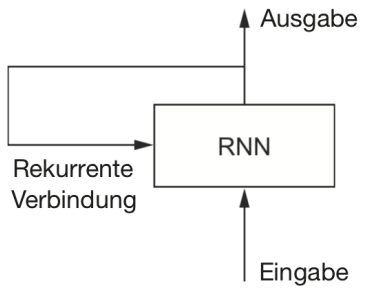
\includegraphics[width=0.5\textwidth,height=4cm,keepaspectratio=true]{content/images/RNNSchleife.png}
    \caption{Schleife in einem \acrshort{rnn} \cite[Abb. 6.9]{DeepLearningPythonKeras}}
    \label{fig:RNNSchleife}
\end{figure}

Ein einfaches \acrshort{rnn} berechnet die Ausgabe $Y_t$ nach \cite[S. 253]{DeepLearningPythonKeras} wie in \autoref{eq:RNN} gezeigt.

\begin{equation}
    Y_t = a(W \cdot X_t + U \cdot S_t + b)
\label{eq:RNN}
\end{equation}

Dabei steht $X_t$ für die Eingabe und $S_t$ für den internen Zustand, jeweils zum Zeitschritt $t$.
$W$ und $U$ sind Matrizen, die die trainierbaren Gewichtungen enthalten und $b$ ist ein trainierbarer Bias-Vektor.
Nach der Berechnung wird die Ausgabe zum neuen internen Zustand, man könnte also $S_t$ in \autoref{eq:RNN} durch $Y_{t-1}$ ersetzen.

Diese einfache Architektur unterliegt nach \cite[S. 260]{DeepLearningPythonKeras} jedoch dem sogenannten \emph{Problem des verschwindenden Gradienten}.
Dieser Effekt sorgt dafür, dass relativ weit zurückliegende Eingaben praktisch keinen Einfluss mehr auf die Ausgabe haben.
Es sind jedoch Anwendungsfälle denkbar, in denen auch weiter zurückliegende Ereignisse einen großen Einfluss auf die Gegenwart haben.
Für die Vorhersage von mobilen Radarkontrollen könnte beispielsweise von Bedeutung sein, wie die Verteilung der Radarkontrollen vor 15 Tagen ausgesehen hat.
Das liegt daran, dass die Daten eine Periodizität von z.B. 15 Tagen aufweisen könnten.

Zur Lösung dieses Problems gibt es verschiedene alternative \acrshort{rnn}-Architekturen.
Eine davon ist \acrfull{lstm}.
Wie der Name vermuten lässt, ermöglicht die \acrshort{lstm}-Architektur, sowohl Abhängigkeiten von weit zurückliegenden als auch aktuellere Eingaben zu lernen.
Die \acrshort{lstm}-Architektur ist in \autoref{fig:LSTMCell} dargestellt.

\begin{figure}[h]
    \centering
    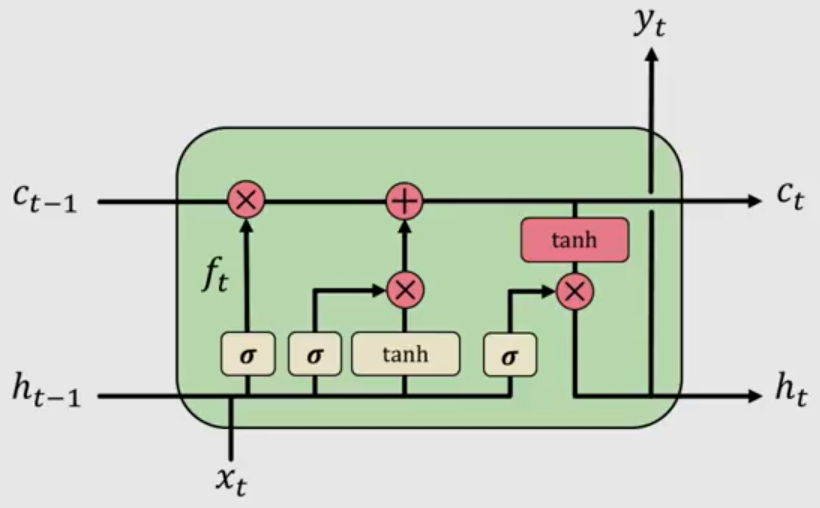
\includegraphics[width=0.8\textwidth,height=6cm,keepaspectratio=true]{content/images/LSTMCell.png}
    \caption{Schematische Darstellung einer \acrshort{lstm}-Zelle \cite{6S191RNN}}
    \label{fig:LSTMCell}
\end{figure}

Eine \acrshort{lstm}-Zelle enthält drei sogenannte Tore (engl. Gates).
Ein Tor ist selbst ein \acrshort{nn}.
Die drei Tore und ihre jeweilige vorgesehene Wirkung sind nach \cite{6S191RNN}:

\begin{enumerate}
    \setlength\itemsep{0.2em}
    \item \textbf{Vergessens-Tor}: Dieses Tor sorgt dafür, dass irrelevante Informationen aus dem vorherigen Zustand "`vergessen"' werden.
    \item \textbf{Merk-Tor}: Dieses Tor fügt dem Zustand relevante neue Informationen hinzu.
    \item \textbf{Ausgangs-Tor}: Dieses Tor bestimmt, welche Informationen aus dem Zustand zum Ausgang der Zelle gelangen sollen.
\end{enumerate}

Amini und Soleimany stellen die vorgesehene Wirkung der Tore in \cite{6S191RNN} ohne weitere kritische Auseinandersetzung dar.
Wie Chollet in \cite[S. 263]{DeepLearningPythonKeras} argumentiert, ist diese Wirkung jedoch keinesfalls garantiert.
Die tatsächliche Wirkung hinge nach Chollet viel mehr von den letzendlich antrainierten Gewichtungen der Tore ab.
Amini und Soleimany sind sich jedoch mit Chollet einig, dass es nicht wichtig ist, die interne Funktionsweise einer \acrshort{lstm}-Zelle im Detail zu verstehen.
Chollet geht noch einen Schritt weiter und argumentiert, dass dies ganz allgemein keine Aufgabe der Menschen sei.
Wichtig ist nach Chollet, Amini und Soleimany nur sich im klaren zu sein, welche Aufgabe eine \acrshort{lstm}-Zelle erfüllt - sie ermöglicht es, sowohl langfristige als auch kurzfristige Zusammenhänge anhand der Trainingsdaten zu erlernen.

\subsection{Faltungsnetze}
\label{sec:CNN}

Mit der bisher vorgestellten \acrshort{lstm}-Architektur können die zeitlichen Zusammenhänge bei der Vorhersage von mobilen Radarkontrollen erlernt werden.
Jedoch wurde bereits motiviert, warum auch räumliche Zusammenhänge für diese Aufgabenstellung von Bedeutung sind.
Prinzipiell ist es möglich, 2D-Daten mit Feedforward-Netzen zu verarbeiten.
Dazu müssen die 2D-Daten verflacht werden.
Für ein zweidimensionales Bild bedeutet das, dass jedes Pixel einem Eingangsneuron zugeführt wird.
Hierbei geht die räumliche Struktur der Daten jedoch verloren.
Das \acrshort{nn} kann nicht wissen, welche Pixel in alle vier Richtungen benachbart waren.
Mit genug Trainingsdaten können einfache Klassifizierungsaufgaben dennoch mit dieser Netzarchitektur bearbeitet werden.
Chollet demonstriert beispielsweise in \cite[S. 53]{DeepLearningPythonKeras}, dass bei der Klassifizierung von handgeschriebenen Ziffern mit einem Feedforward-Netz eine Korrektklassifizierungsrate von 97,8\,\% erreicht werden kann.
Das Problem mit Feedforward-Netzen ist jedoch, dass sie nur globale Muster erlernen, also beispielsweise eine Ziffer als Ganzes.
Ist dieselbe Ziffer nun etwas im Bild verschoben oder auf sonstige Weise verzerrt, wird sie von einem Feedforward-Netz nicht mehr erkannt.
Dies kann dadurch visualisiert werden, dass nach einer Verzerrung die einzelnen Pixel an ganz anderen Eingangsneuronen anliegen.

Abhilfe hierbei verschaffen Faltungsnetze (engl. \acrlongpl{cnn}, \acrshortpl{cnn}).
\acrshortpl{cnn} entsprechen dem Stand der Technik, wenn es um die Verarbeitung von 2D-Daten geht.
Wenn das vorherige Beispiel nochmals betrachtet wird, kann man erkennen, welche Eigenschaften der Ziffern sich nicht durch eine Verzerrung ändern: Die Zusammensetzung der Ziffern aus kleineren Merkmalen.
Selbst wenn eine Ziffer verschoben oder leicht verzerrt wird, werden sich (relativ zueinander) immer noch dieselben Linien an denselben Stellen kreuzen oder berühren.
Die Betrachtung von 2D-Daten als Zusammensetzung von lokalen Mustern wird in \autoref{fig:LokaleMuster} verdeutlicht.

\begin{figure}[h]
    \centering
    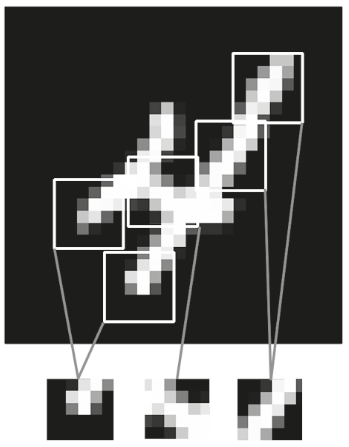
\includegraphics[width=0.4\textwidth,height=4cm,keepaspectratio=true]{content/images/LokaleMuster.png}
    \caption{Lokale Muster wie Ränder und Linien in einer handgeschriebenen Ziffer \cite[Abb. 5.1]{DeepLearningPythonKeras}}
    \label{fig:LokaleMuster}
\end{figure}

\acrshortpl{cnn} erkennen nach \cite[S. 164]{DeepLearningPythonKeras} nun diese lokalen Muster.
Chollet geht in \cite{DeepLearningPythonKeras} auf Seite 165 auf die daraus resultierenden Eigenschaften von \acrshortpl{cnn} ein.
Zunächst sei die Erkennung der lokalen Muster translationsinvariant.
Dies bedeute, dass die Muster an beliebigen Stellen im Bild erkannt werden können.
Außerdem könne durch das Hintereinanderschalten mehrer \acrshort{cnn}-Layer erreicht werden, dass Hierarchien von Mustern erlernt werden.
Aus diesen beiden Eigenschaften folgt, dass es für ein \acrshort{cnn} keinen Unterschied macht, ob die zu erkennenden globalen Muster (beispielsweise eine Ziffer) in der Eingabe verschoben sind.

Als Nächstes stellt sich die Frage, wie \acrshortpl{cnn} lokale Muster erkennen können.
Dies wird durch die Faltungsoperation erreicht.
Die Idee der Faltungsoperation ist nach \cite{6S191CNN}, einen sogenannten Filter zu verwenden, der lokale Muster erkennt.
Dieser zweidimensionale Filter wird über die 2D-Eingabe "`geschoben"' und erkennt somit, wo sich in der Eingabe ein bestimmtes Muster befindet.
Mathematisch gesehen ist ein Filter eine quadratische Matrix.
Die Elemente der Matrix sind die erlernbaren Gewichtungen, die je nach ihren Werten verschiedene Muster erkennen.
Die Erkennung geschieht dadurch, dass der Filter an der jeweiligen Stelle komponentenweise mit der Eingabe multipliziert und die einzelnen Werte anschließend aufsummiert werden.
Diese Berechnung wird in \autoref{fig:ConvExample} verdeutlicht.

\begin{figure}[h]
    \centering
    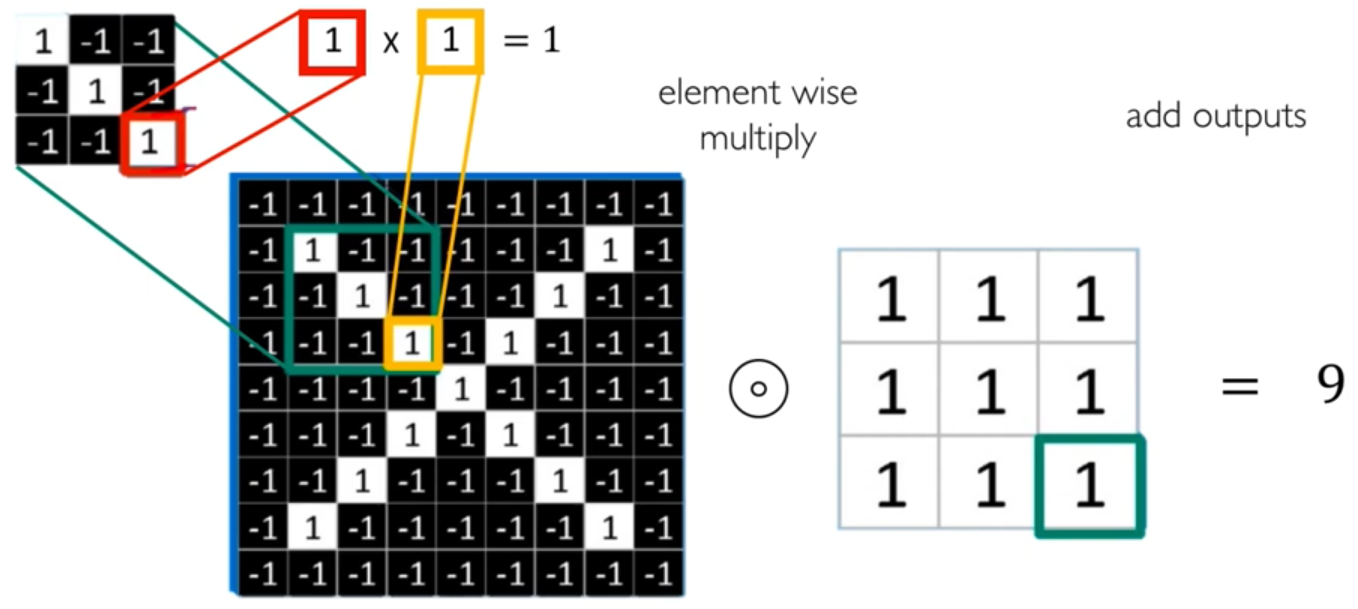
\includegraphics[width=1.0\textwidth,height=8cm,keepaspectratio=true]{content/images/ConvExample.png}
    \caption{Ein Schritt der Faltung des Filters mit der Eingabe \cite{6S191CNN}}
    \label{fig:ConvExample}
\end{figure}

Links oben in der Abbildung ist der Filter dargestellt.
Dieser Filter erkennt schräge Linien von links oben nach rechts unten.
Bei einer perfekten Übereinstimmung, wie im Beispiel der Abbildung, wird das Ergebnis der Berechnung maximal.
Angenommen, das Pixel oben in der Mitte der Eingabe wäre $1$, dann wäre das Ergebnis der Berechnung nur $7$.
Der Wert des Ergebnisses ist also ein Maß für die Übereinstimmung des Filters mit der Eingabe.
Auf dieses Ergebnis wird in der Praxis nach \cite{6S191CNN} noch eine Aktivierungsfunktion angewendet, wofür meistens \emph{\acrshort{relu}} verwendet wird.
Negative Pixel werden dadurch zu null.
Wird der Filter nun mit einer Schrittweite von $1$ in $x$- und $y$-Richtung über die gesamte Eingabe geschoben und die Berechnung jedes Mal ausgeführt, entsteht eine sogenannte Merkmalskarte (engl. \emph{feature map}).
Die Merkmalskarte gibt an, wo im Bild die Übereinstimmung mit dem durch den Filter beschriebenen Muster wie groß ist.
Damit die Merkmalskarte die gleiche Höhe und Breite wie die Eingabe hat, kann nach \cite[S. 168 f.]{DeepLearningPythonKeras} die Eingabe vor der Faltungsoperation rundherum mit Nullen aufgefüllt werden.
Dies wird auch \emph{Padding} genannt.

Nach der Faltungsoperation ist noch ein weiterer wichtiger Schritt notwendig.
Da die Merkmalskarte zunächst die gleichen Dimensionen wie die Eingabe hat, können nach \cite[S. 171]{DeepLearningPythonKeras} keine Merkmalshierarchien erkannt werden.
Das liegt daran, dass ein Pixel der Merkmalskarte nur Informationen über einen Bereich der Eingabe enthält, der so groß ist wie der Filter.
In den meisten Fällen sind dies nur 3x3 oder 5x5 Pixel.
Das Ziel ist es also, eine Merkmalskarte zu erstellen, bei der ein Pixel Informationen über einen größeren Bereich der Eingabe enthält.
Dies kann durch die MaxPooling-Operation erreicht werden, die auf die Merkmalskarte angewendet wird.
Diese funktioniert ähnlich wie die Faltungsoperation.
Auch hier gibt es einen Filter, der über die Eingabe geschoben wird.
Dieser Filter wird hier jedoch als \emph{Pool} bezeichnet.
Im Gegensatz zur Faltungsoperation wird nichts multipliziert.
Stattdessen entspricht die Ausgabe des Pools dem Maximalwert der Eingabe.
Hat der Pool beispielsweise eine Größe von 2x2 und wird in $x$- und $y$-Richtung jeweils um die Schrittweite $2$ verschoben, wird die Seitenlänge der Eingabe durch die MaxPooling-Operation halbiert.
Dies wird in \autoref{fig:MaxPooling} an einem Beispiel veranschaulicht.

\begin{figure}[h]
    \centering
    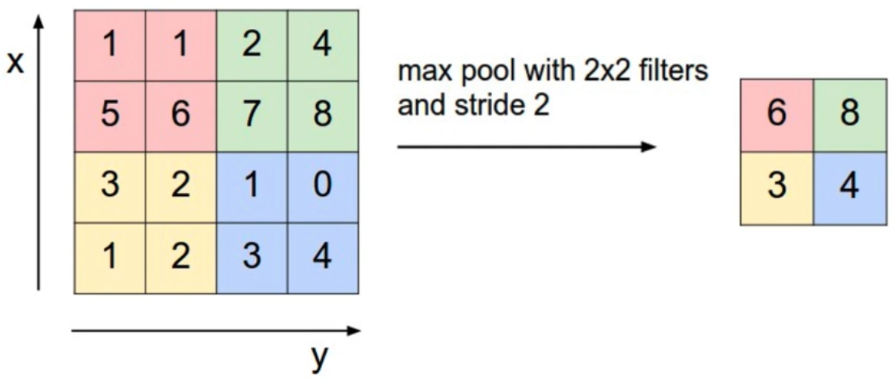
\includegraphics[width=0.8\textwidth,height=8cm,keepaspectratio=true]{content/images/MaxPooling.png}
    \caption{Beispiel einer MaxPooling-Operation \cite{6S191CNN}}
    \label{fig:MaxPooling}
\end{figure}

Werden mehrere \acrshort{cnn}- und MaxPooling-Layer abwechselnd hintereinandergeschaltet, lassen sich die Merkmale der Eingabe hierarchisch darstellen.
Dabei wird die Höhe und Breite der Eingabe nach jedem MaxPooling-Layer halbiert.
Zumm Schluss wird die Ausgabe des letzten MaxPooling-Layers an ein Feedforward-Netz zur Klassifizierung übergeben.
Das Feedforward-Netz klassifiziert die Eingabe also nun anhand von abstrakten Merkmalen, die durch die \acrshort{cnn}- und MaxPooling-Layer von \emph{beliebigen Stellen} in der Eingabe extrahiert wurden.

\subsection{Verwantete Forschung}
\label{sec:VerwanteteForschung}





\section{Vorverarbeitung des Datensatzes}
\label{sec:Datensatz}
In diesem Kapitel wird zunächst eine erste Analyse des Datensatzes durchgeführt, um diesen auf Plausibilität zu überprüfen.
Anschließend wird erörtert, wie die Datenpunkte möglichst effizient in ein Raster umgewandelt werden können.

\subsection{Analyse und Aufbereitung}
\label{sec:AnalyseAufbereitung}

Ziel dieses Abschnitts ist es, sich mit dem Datensatz vertraut zu machen und ihn aufzubereiten, sodass beispielsweise ungültige Einträge gelöscht werden.
Außerdem ist es sinvoll, einige Analysen durchzuführen.
Dies führt zu einem besseren Verständnis des Datensatzes und legt etwaige Inkonsitenzen offen.

Der von der Eifrig Media GmbH bereitgestellte Datensatz liegt als sql-Datei vor.
Für die Weiterverarbeitung muss die Datei in eine MySQL oder MariaDB Datenbank eingelesen werden.
Die Datenbank kann komfortabel mit Docker erstellt werden.
Eine entsprechende Docker-Compose Datei mit einer MariaDB Instanz und weiteren Komponenten, die im Verlauf dieses Abschnitts benötigt werden, befindet sich im Anhang in \autoref{lst:DockerComposeDBs}.
Als grafische Oberfläche für den Zugriff auf die Datenbank enthält die Docker-Compose Datei eine phpMyAdmin Instanz.

Bei Betrachtung des Datensatzes fällt zunächst auf, dass einige Meldungen Inkonsistenzen aufweisen:

\begin{itemize}
    \setlength\itemsep{-15pt}
    \item 1160 Meldungen haben als Aufbauzeitpunkt den ungültigen Wert "`0000-00-00 00:00:00"'.
    \item Bei 420 Meldungen liegt das Abbauzeitpunkt vor dem Aufbauzeitpunkt.
    \item Bei 9800 Meldungen beträgt die Standdauer 20 Minuten oder weniger.
    \item Bei 62.000 Meldungen beträgt die Standdauer mehr als 24 Stunden, bei 1960 mehr als ein Jahr.
\end{itemize}

Da der Anteil an Meldungen mit ungültigem Auf- oder Abbaudatum nur 0,02\% beträgt, bietet es sich an, diese Meldungen aus dem Datensatz zu entfernen.
Auch die Meldungen mit einer sehr geringen Standdauer von 20 Minuten oder weniger sollten entfernt werden, da es sich hierbei vermutlich um Fehlmeldungen handelt.
Nun stellt sich die Frage, wie mit Meldungen umgegangen werden soll, die eine sehr lange Standdauer aufweisen.
Da sich im Datensatz 1962 Meldungen befinden, deren Standdauer über ein Jahr beträgt, ist davon auszugehen, dass die Standdauer einiger Meldungen im Datensatz falsch ist.
Aus Erfahrung kann gesagt werden, dass schon eine Standdauer von mehr als 12 Stunden in der Realität sehr selten auftritt.
Der Datensatz enthält jedoch ca. 91.000 Meldungen, auf die dieses Kriterium zutrifft.
Dies entspricht einem Anteil von 1,1 \%, was zu groß ist, um diese Meldungen komplett aus dem Datensatz zu entfernen.
Die bevorzugte Alternative besteht darin, den Abbauzeitpunkt aller dieser Meldungen auf 12 Stunden nach dem Aufbauzeitpunkt zu setzen.
Eine weitere Inkonsistenz fällt auf, wenn die Anzahl der Meldungen pro Tag über den gesamten Zeitraum des Datensatzes betrachtet.
Diese Metrik ist in \autoref{fig:AnzahlProTagAllData} dargestellt.

\begin{figure}[h]
    \centering
    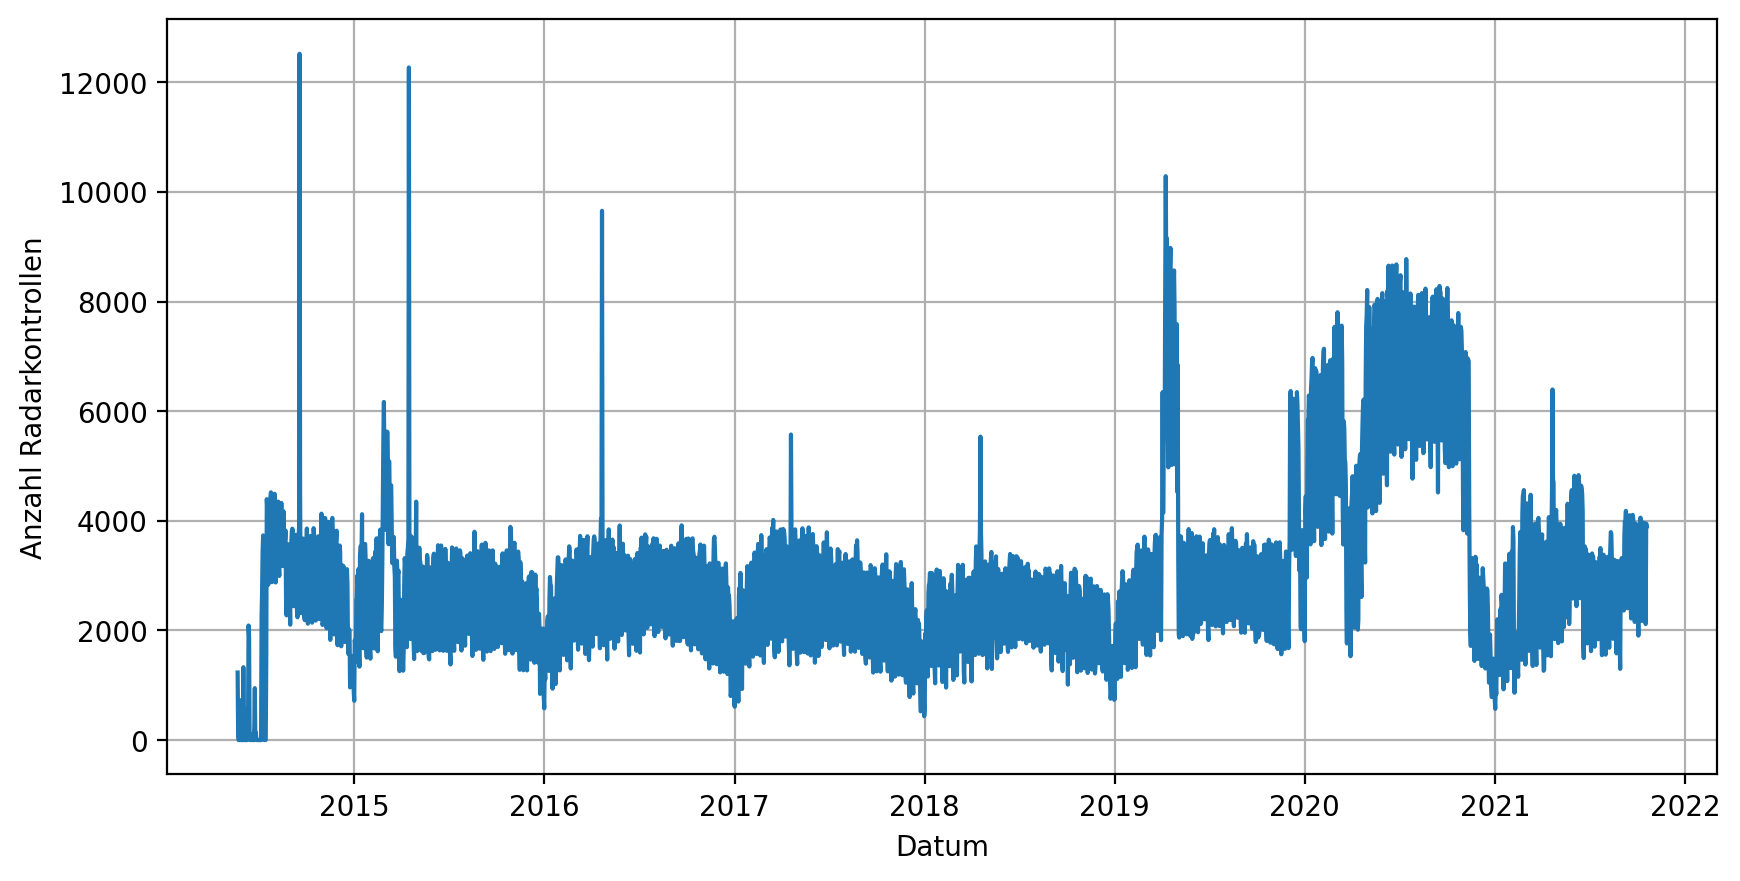
\includegraphics[width=1.0\textwidth,height=10cm,keepaspectratio=true]{content/images/AnzahlProTagAllData.png}
    \caption{Anzahl mobiler Radarkontrollen pro Tag vom 22.05.2014 bis 20.10.2021}
    \label{fig:AnzahlProTagAllData}
\end{figure}

Es fällt auf, dass deutlich weniger Meldungen im Zeitraum vom 22.05.2014 bis zum 16.07.2014 vorhanden sind als in den Jahren danach.
Das spricht dafür, dass der Datensatz in diesem Zeitraum unvollständig ist.
Da dies das Training des \acrshort{nn}s negativ beeinflussen würde, sollten alle Meldungen vor dem 17.07.2014 aus dem Datensatz entfernt werden.
In \autoref{fig:AnzahlProTagAllData} sind noch einige interessante Muster zu erkennen.
Zunächst gibt es einige sehr schmale Ausschläge.
Beispielsweise waren am 17.09.2014 3800 mobile Radarkontrollen aufgestellt, am 18.09.2014 dann 12.400 und am 19.09.2014 wieder nur 4140.
Diese Ausschläge sind je auf einen sogenannten "`Blitzermarathon"' zurückzuführen, bei denen an einem bestimmten Tag besonders viele Radarkontrollen aufgestellt werden.
Ein Vergleich der Radarkontrollen auf einer Karte zwischen dem Blitzermarathon am 18.09.2014 und dem Vortag befindet sich in \appendixref{sec:AnhangDiagramme}, \autoref{fig:BlitzerMarathonSep2014Vgl}.

Als nächstes ist an \autoref{fig:AnzahlProTagAllData} noch auffällig, dass es eine jährliche Periodizität gibt.
Außerdem bleibt die durchschnittliche Anzahl an Radarkontrollen pro Jahr annähernd konstant, wenn der Ausschlag im Jahr 2020 außer Acht gelassen wird.
Das spricht dafür, dass der Datensatz vermutlich nicht durch eine sich verändernde Nutzerzahl verzerrt ist.
Es ist auch erkennbar, dass es im Sommer mehr mobile Radarkontrollen gibt als im Winter.
Dies geht auch aus \autoref{fig:AnzahlNachMonat} hervor, in der die Anzahl mobiler Radarkontrollen pro Monat dargestellt ist.

\begin{figure}[h]
    \centering
    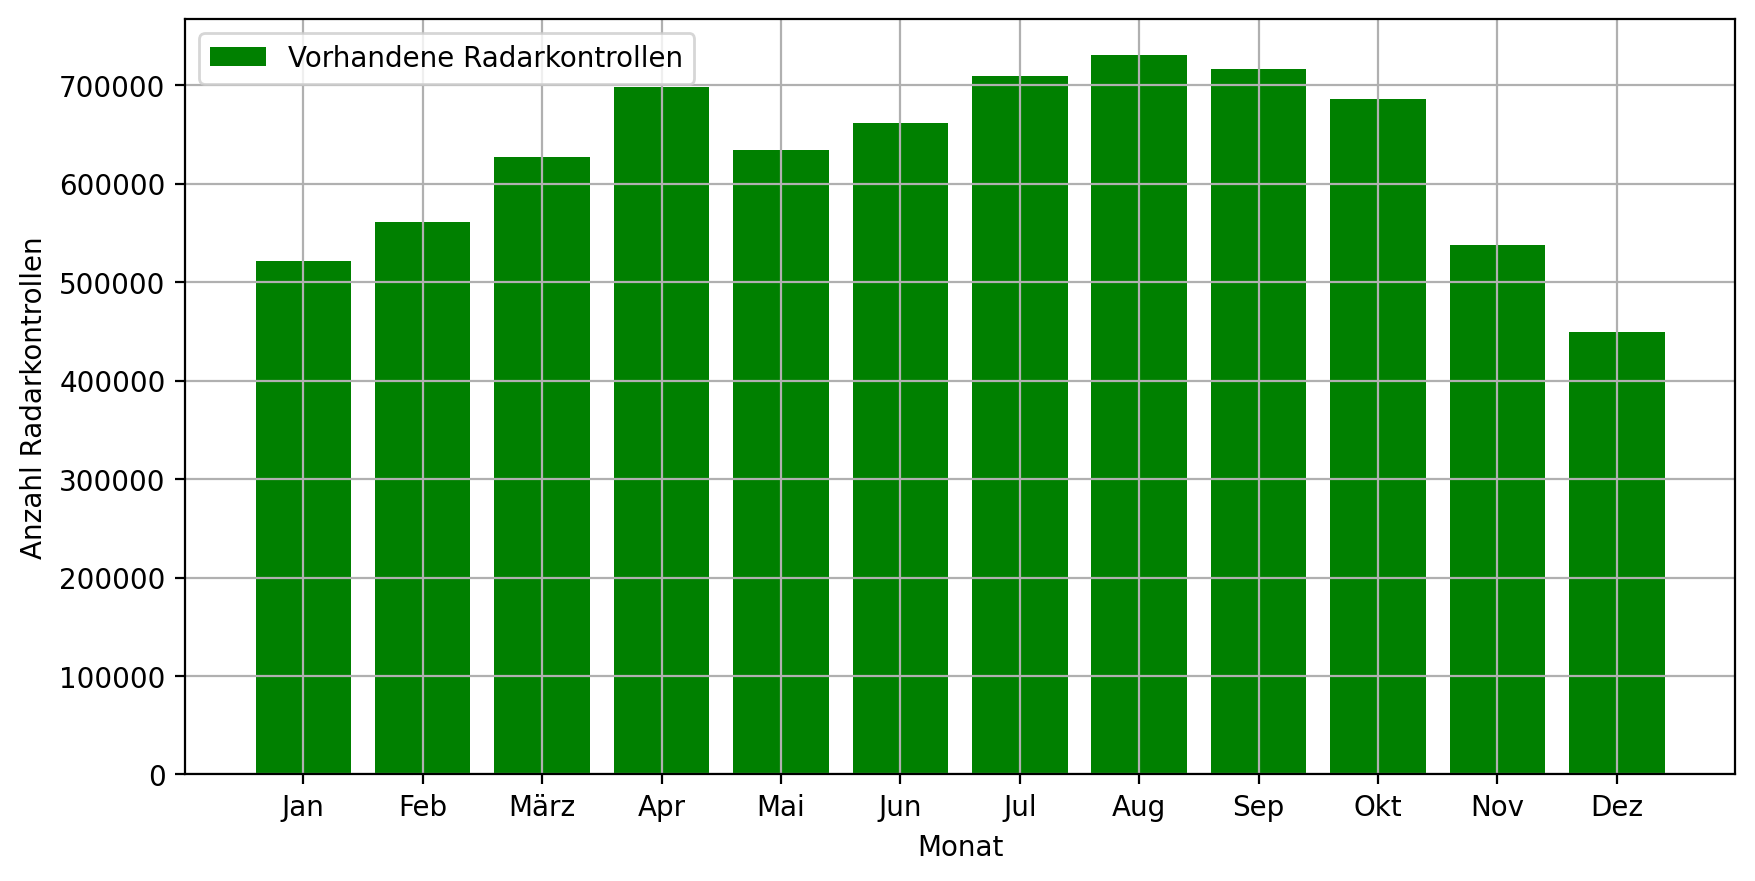
\includegraphics[width=1.0\textwidth,height=10cm,keepaspectratio=true]{content/images/AnzahlNachMonat.png}
    \caption{Anzahl mobiler Radarkontrollen nach Monat}
    \label{fig:AnzahlNachMonat}
\end{figure}





\begin{figure}[h]
    \centering
    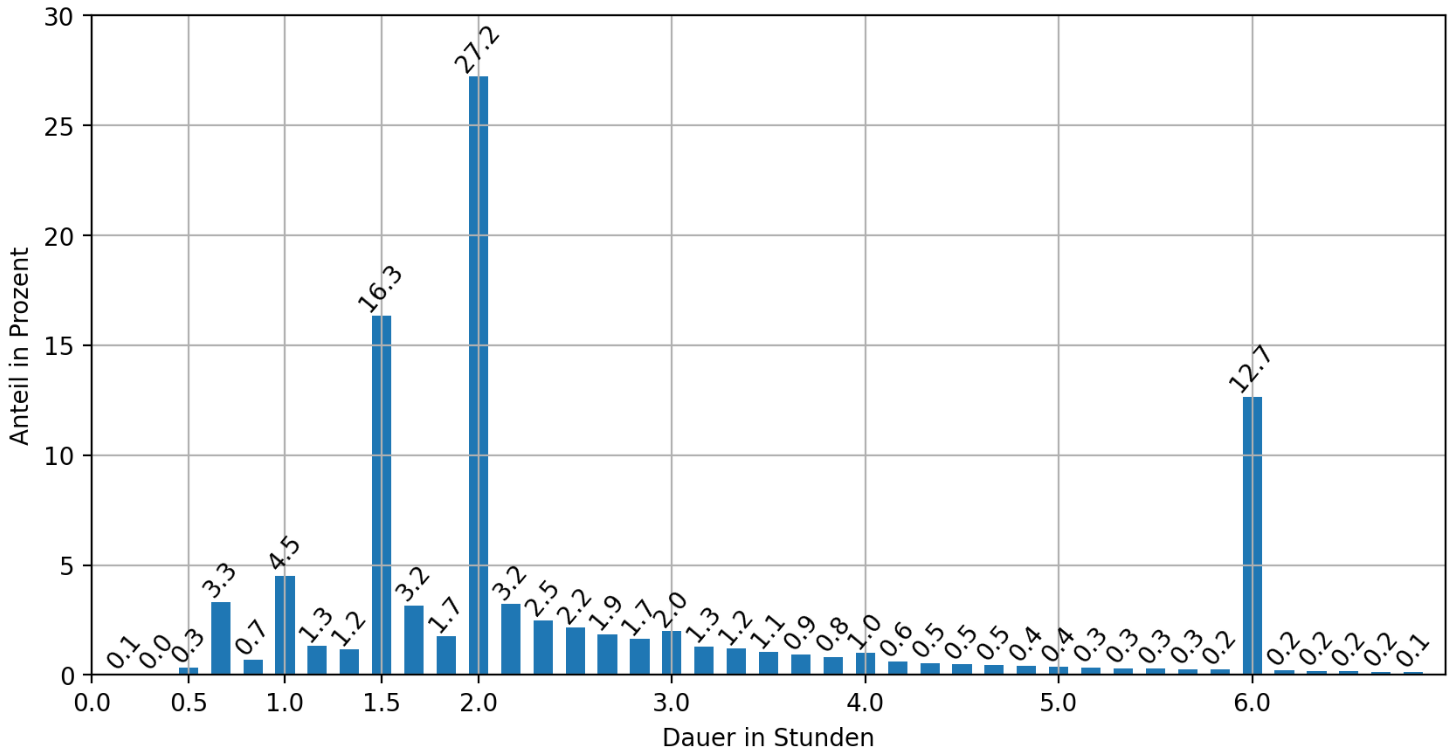
\includegraphics[width=1.0\textwidth,height=10cm,keepaspectratio=true]{content/images/Standdauer.png}
    \caption{Verteilung der Standdauer mobiler Radarkontrollen}
    \label{fig:Standdauer}
\end{figure}

\begin{figure}[h]
    \centering
    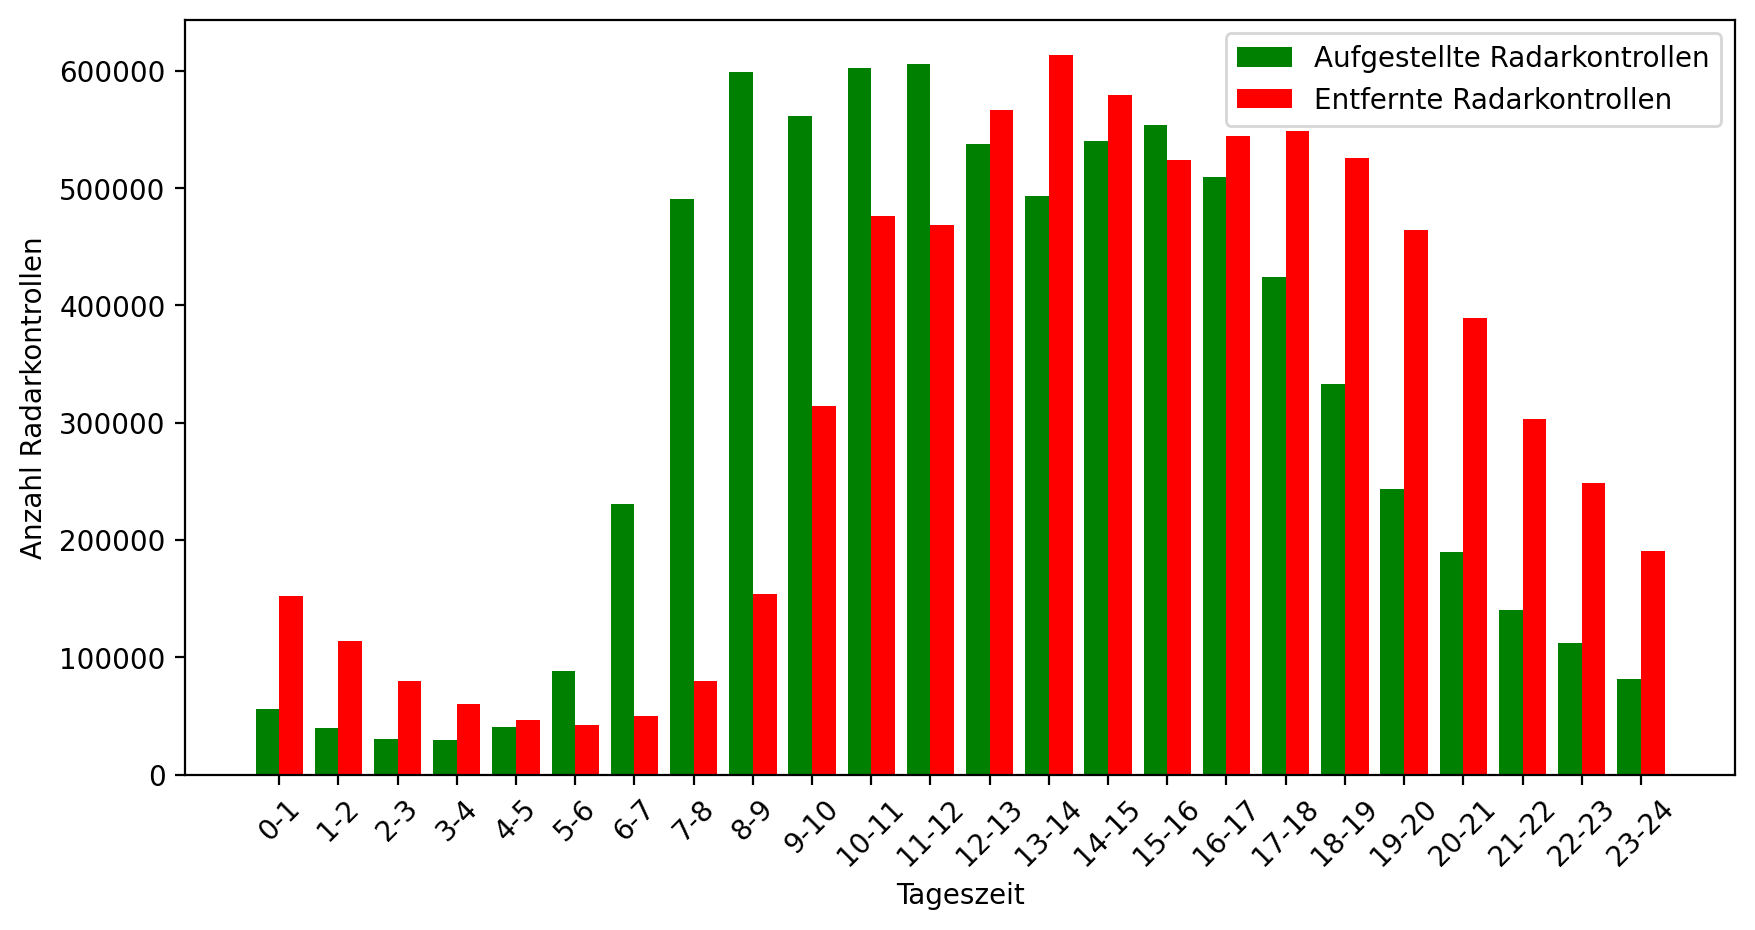
\includegraphics[width=1.0\textwidth,height=10cm,keepaspectratio=true]{content/images/AufbauAbbau.png}
    \caption{Auf- und Abbau mobiler Radarkontrollen nach Tageszeit}
    \label{fig:AufbauAbbau}
\end{figure}

\begin{figure}[h]
    \centering
    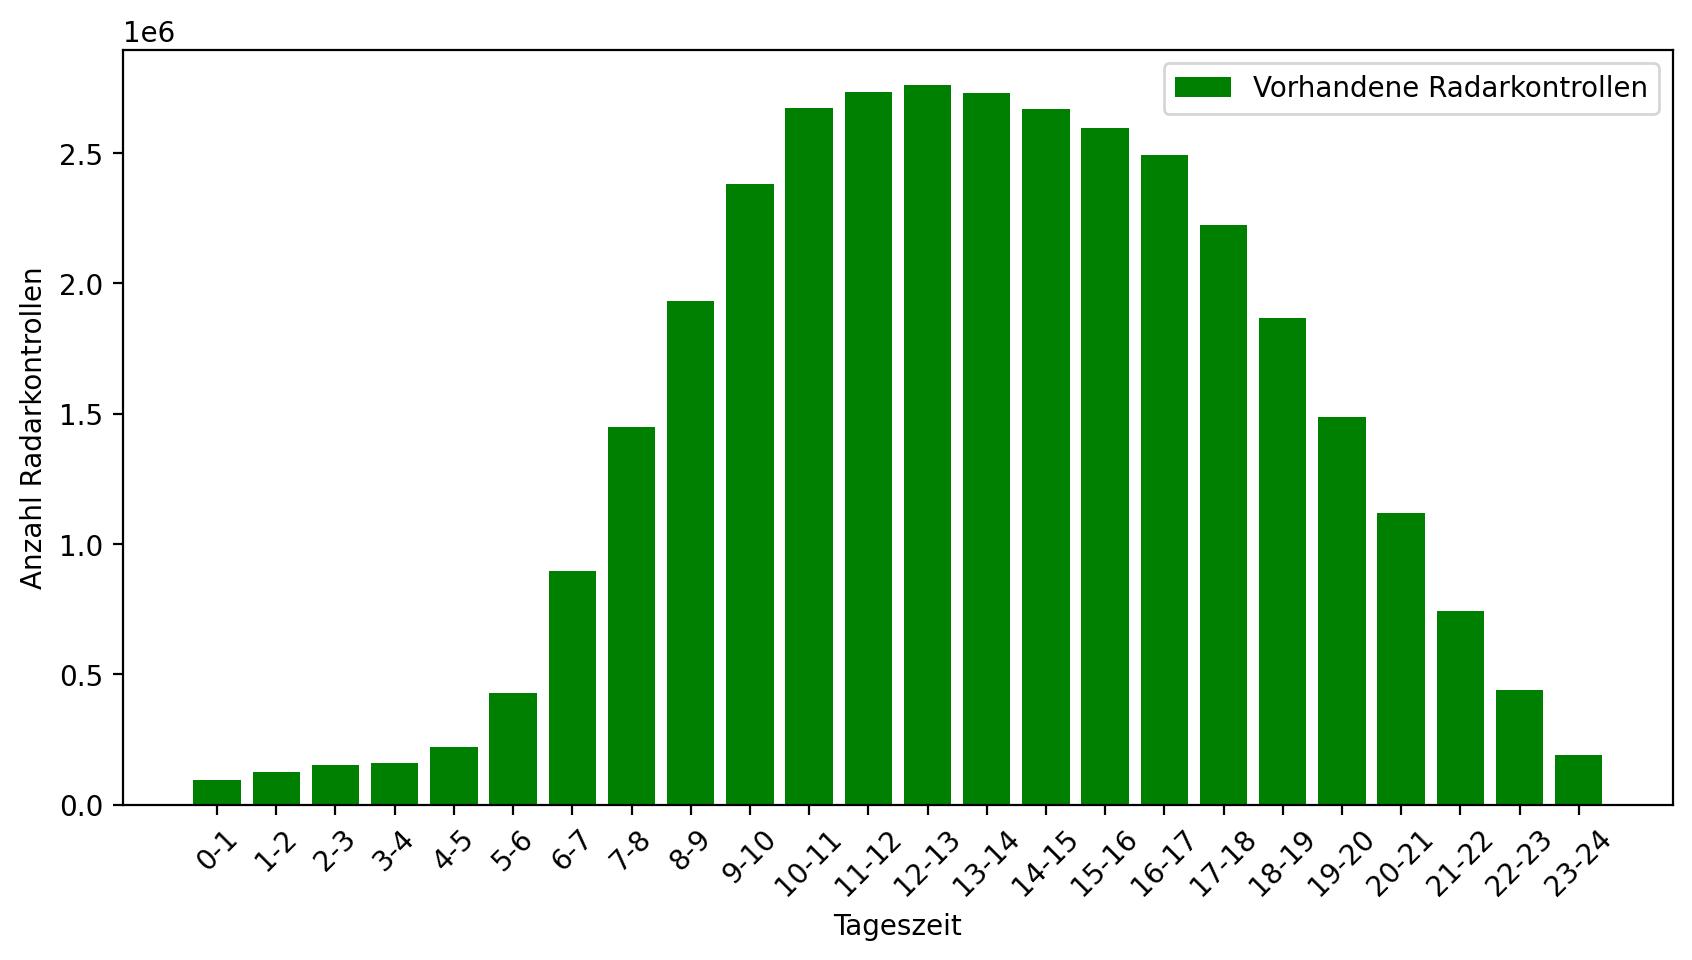
\includegraphics[width=1.0\textwidth,height=10cm,keepaspectratio=true]{content/images/AnzahlNachTageszeit.png}
    \caption{Anzahl mobiler Radarkontrollen nach Tageszeit}
    \label{fig:AnzahlNachTageszeit}
\end{figure}

\begin{figure}[h]
    \centering
    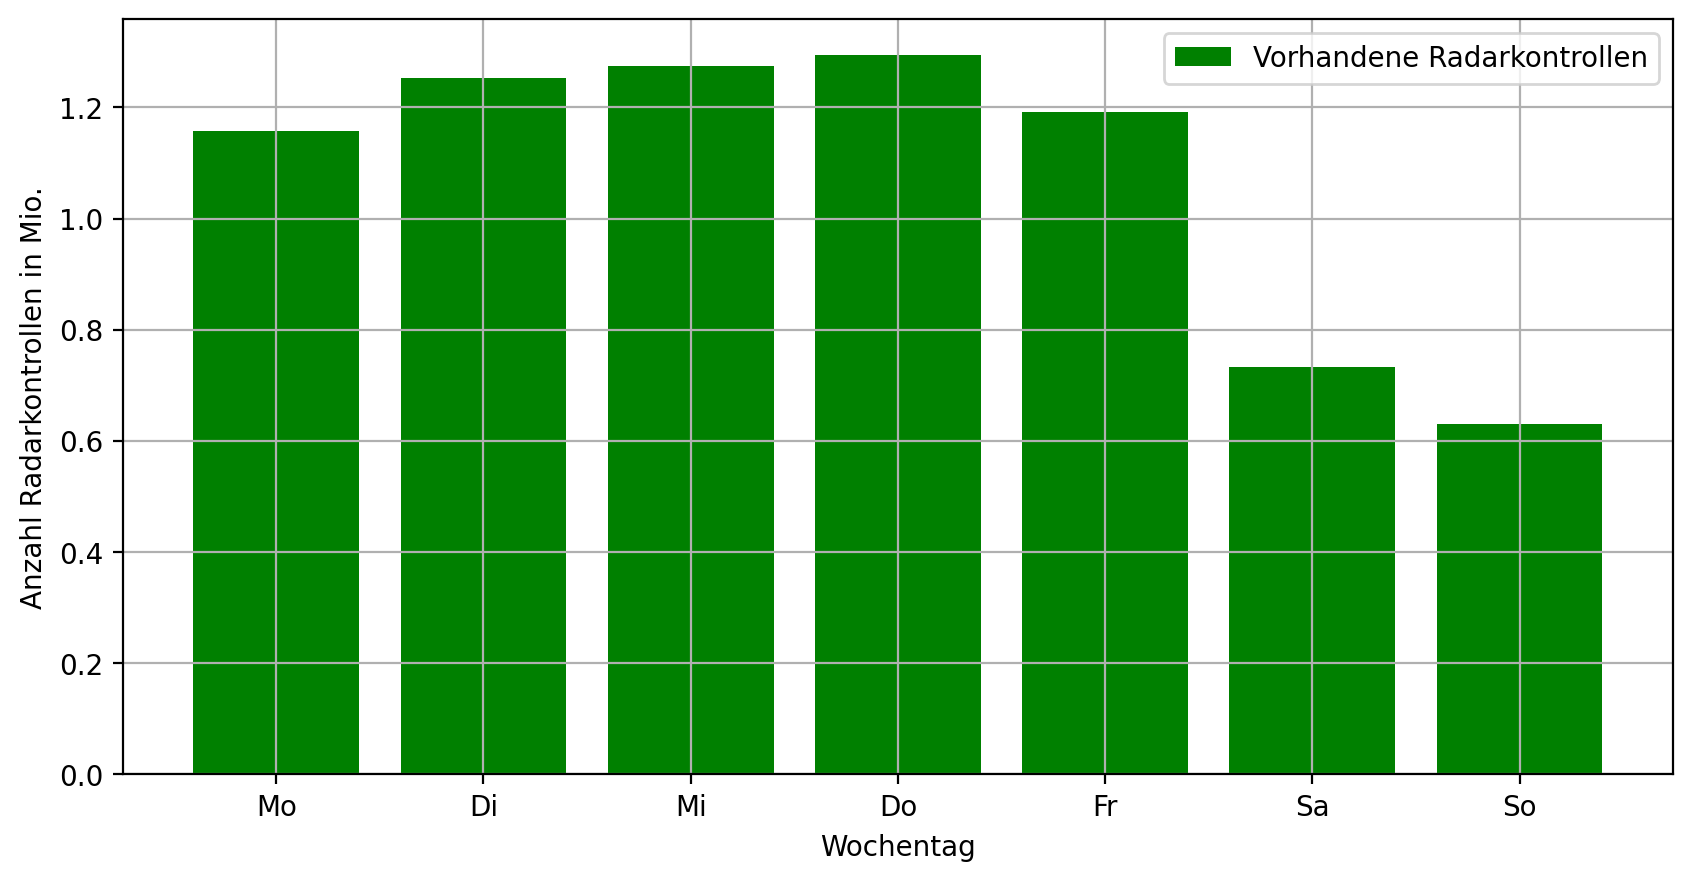
\includegraphics[width=0.8\textwidth,height=8cm,keepaspectratio=true]{content/images/AnzahlNachWochentag.png}
    \caption{Anzahl mobiler Radarkontrollen nach Wochentag}
    \label{fig:AnzahlNachWochentag}
\end{figure}

\subsection{Rasterisierung}
\label{sec:Rasterisierung}
Um ein rasterbasiertes Modell wie ConvLSTM oder ST-ResNet für die Vorhersage von mobilen Radarkontrollen verwenden zu können, müssen die räumlich und zeitlich kontinuierlichen Datenpunkte aus dem Datensatz zunächst rasterisiert werden.
Dazu ist es sinnvoll nochmals zu betrachten, wie die Daten ursprünglich vorliegen.
Jede Meldung ist eine Zeile in einer Datenbanktabelle mit den Spalten \emph{Längengrad}, \emph{Breitengrad}, \emph{Aufbauzeitpunkt} und \emph{Abbauzeitpunkt}.
Das Ziel besteht darin, die Datenpunkte so zu verarbeiten, dass pro Zeitraum $T$ ein Raster aus $n \times n$ quadratischen Zellen mit der Seitenlänge $k$ entsteht, bei dem jeder Zelle ein Wert $x$ zugeordnet ist, der etwas über die gemeldeten Radarkontrollen in dieser Zelle aussagt.
Die Werte $T,~n,~k$ sind hierbei variable Hyperparameter und müssen möglichst sinnvoll ausgewählt werden.
Außerdem muss festgelegt werden, nach welcher Regel der Wert $x$ berechnet werden soll.

\subsubsection{Auswahl der Parameter zur Rasterisierung}
\label{sec:RasterisierungParameter}
Bei der Auswahl des Zeitraums $T$ muss zwischen der gewünschten zeitlichen Genauigkeit und der Anzahl an verfügbaren Datenpunkten abgewägt werden.
Wird $T$ beispielsweise zu klein gewählt, enthält der betrachtete Bereich zu wenige Meldungen, um auf deren Basis aussagekräftige Vorhersagen treffen zu können.
Wird $T$ hingegen zu groß gewählt (wie z.\,B. eine Woche oder ein Monat), haben die Vorhersagen weniger praktischen Nutzen.
Außerdem könnten dann insgesamt zu wenige Zeitschritte vorliegen, um das Modell trainieren zu können.
Nach einigen Versuchen scheinen 24 Stunden für $T$ ein guter Wert zu sein, da somit der praktische Nutzen erhalten bleibt und es dennoch genug Meldungen pro Zeitschritt gibt.

Als Nächstes sind $k$ udn $n$ zu wählen.
Die Seitenlänge des gesamten betrachteten Bereichs berechnet sich daraus mit $n \cdot k$.
Bei der Wahl von $k$ muss dieselbe Abwägung getroffen werden wie bei der Wahl von $T$, jedoch geht es hier um den praktischen Nutzen der Vorhersagen je nach räumlicher Auflösung.
Wird $k$ zu groß gewählt, ist die zeitliche Auflösung zu gering, als dass die Vorhersagen nützlich wären.
Wenn $k$ hingegen zu klein gewählt wird, gibt es in zu wenigen Zellen eine Meldung, um das Modell gut trainieren zu können.
Bei der Wahl von $k$ kommt es außerdem darauf an, ob eher städtischer oder ländlicher Raum betrachtet werden soll.
Für den ländlichen Raum scheint $k = 4~\text{km}$ eine gute Wahl zu sein, da die Radarkontrollen dort nicht sonderlich dicht liegen.
Für den städtischen Raum ist dieser Wert jedoch zu groß, da sich in einem 4 km Radius vergleichsweise deulich mehr Straßen befinden.
Außerdem ist die Dichte an Radarkontrollen im städtischen Raum höher, weshalb ein geringeres $k$ von einem oder zwei Kilometer durchaus möglich ist.
Wird (beispielsweise in Baden-Württemberg) insgesamt ein größerer Raum abgedeckt, besteht die meiste Fläche aus ländlichem Gebiet.
Daher wird im folgenden mit $k = 4~\text{km}$ fortgefahren.
Die Wahl von $n$ beeinflusst nun den insgesamt durch das Raster abgedeckten Raum.
Optimalerweise sollte dieser Wert möglichst groß sein, um möglichst viele Trainingsdaten einzuschließen.
Andererseits ist $n$ durch den während des Trainings verfügbaren Speicher begrenzt.
Wird das Training auf einer Grafikkarte ausgeführt, müssen das komplette Modell und alle Trainingsdaten, die pro Batch verarbeitet werden in den Grafikspeicher passen.
Da der Speicherbedarf quadratisch mit $n$ ansteigt, ist man hier in der Praxis sehr eingeschränkt.
Bei einem Grafikspeicher von 8 GB und einer Batch Size von 12 ist $n = 50$ gut möglich.
Mit $k = 4~\text{km}$ ergibt sich dann eine Seitenlänge des gesamten Rasters von 200 km.

Für die Berechnung von $x$ gibt es mehrere Möglichkeiten.
Zunächst könnte $x = 1$ gesetzt werden, wenn sich in der Zelle mindestens eine Radarkontrolle befindet, ansonsten $x = 0$.
Alternativ kann $x$ auf die Anzahl der Radarkontrollen gesetzt werden, die sich im jeweiligen Zeitraum in der Zelle befinden.
Dies hat jedoch den Nachteil, dass eine Radarkontrolle mit einer kurzen Standdauer gleich gewichtet wird wie eine Radarkontrolle mit einer deutlich längeren Standdauer.
Daher bietet es sich an, die Standdauer aller Radarkontrollen in einer Zelle aufzusummieren.
Mit dieser Möglichkeit enthält $x$ am meisten Informationen über die Radarkontrollen in der jeweiligen Zelle.
Es entsteht dadurch eine Heatmap, die die Signifikanz der Radarkontrollen pro Rasterzelle darstellt.
Außerdem kann diese Repräsentation auch nach der Rasterisierung einfach in eine binäre Unterscheidung umgewandelt werden, indem pro Zelle $x := x > 0$ gesetzt wird.

\subsubsection{Auswahl von Methoden und Tools zur Rasterisierung}
\label{sec:RasterisierungMethodenTools}
Nun stellt sich die Frage, wie die Rasterisierung mit den erörterten Parametern möglichst effizient ausgeführt werden kann.
Die einfachste Möglichkeit besteht darin, alle Meldungen pro Rasterzelle und Datum nacheinander mit einem Python-Skript von der MariaDB-Datenbank abzufragen.
Pro Rasterzelle dauert diese Abfrage ca. 0,32 Sekunden.
Bei 200 Zellen und 2648 Tagen würde die Rastergenerierung damit jedoch 47 Stunden dauern, was unpraktikabel ist.
Eine mögliche Optimierung ist, eine Geodatenbank zu verwenden, die das Filtern nach Koordinaten effizienter ausführen kann als MariaDB.
Eine solche Geodatenbank ist PostgreSQL mit der Erweiterung PostGIS.
Die Abkürzung \acrshort{gis} in PostGIS steht für \acrlong{gis}.
Dies ist ein Begriff für Systeme, die besonders auf die Verarbeitung von räumlichen Daten optimiert sind, wozu auch Geodatenbanken gehören.
Eines der wichtigsten Features einer Geodatenbank ist ein räumlicher Index (engl. \emph{spatial index}).
Ein solcher ist laut \cite[S. 2707 f.]{SpatialIndexingTechniques} eine Datenstruktur, die einen schnelleren Zugriff auf räumliche Daten bietet als traditionelle eindimensionale Indexe wie ein B\textsuperscript{+}-Baum.
Ein bekanntes Beispiel für einen räumlichen Index ist der R-Baum, der auch von PostGIS verwendet wird \cite{PostGISSpatialIndex}.
Die Funktionsweise eines R-Baums ist in \autoref{fig:RTreeImage} dargestellt.

\begin{figure}[h]
    \centering
    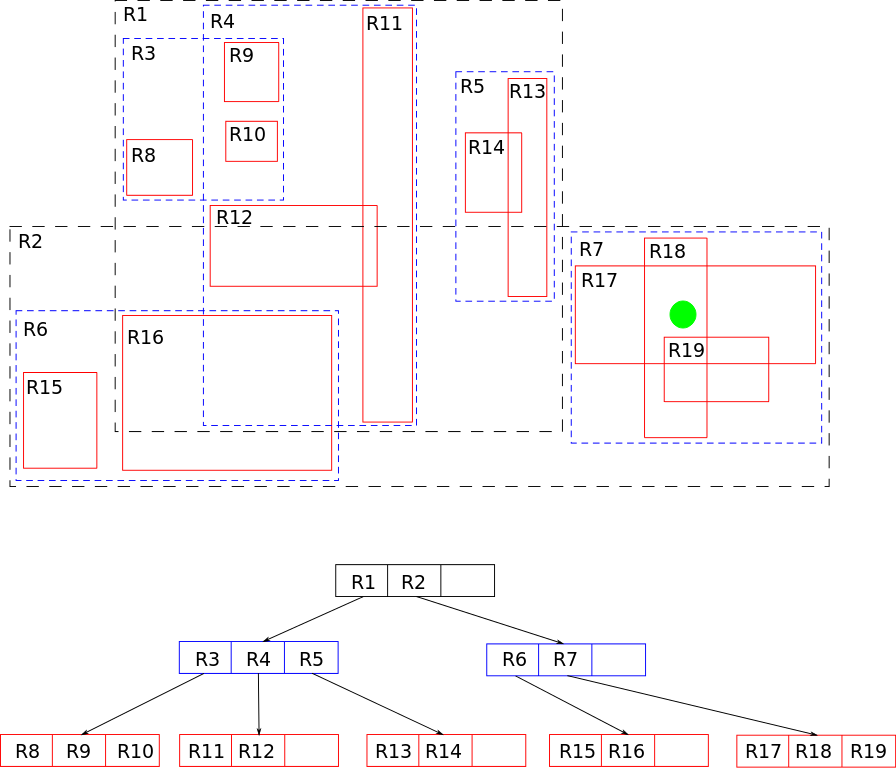
\includegraphics[width=1.0\textwidth,height=10cm,keepaspectratio=true]{content/images/R-tree.png}
    \caption{Aufbau und Funktionsweise eines R-Baums \cite{RTreeImage}}
    \label{fig:RTreeImage}
\end{figure}

Wie in der Abbildung zu erkennen ist, enthält jeder Knoten eines R-Baums Informationen über ein Rechteck.
Die Knoten können dann nach \cite{RTrees} jeweils Kindknoten haben, deren Recktecke komplett innerhalb des Rechtecks des Elternknotens liegen müssen.
Als Beispiel für die Suchoperation auf einem R-Baum sollen alle Rechtecke R8 bis R19 ermittelt werden, die sich mit dem in \autoref{fig:RTreeImage} grün markierten Punkt überschneiden.
Ohne den R-Baum müssten alle 12 Recktecke R8 bis R19 nacheinander mit dem Punkt verglichen werden.
Mit dem R-Baum sind nur noch sieben Vergleiche notwendig.
Zunächst wird ermittelt, ob der Punkt in R1 oder R2 liegt.
Da der Punkt in R2 liegt, können R8 bis R14 nun schon ausgeschlossen werden.
Daraufhin wird der Punkt mit R6 und R7 verglichen.
Da der Punkt in R7 liegt, liefern die Vergleiche mit R17, R18 und R19, dass sich nur R17 und R18 mit dem Punkt überschneiden.
Dieser Performancegewinn macht sich nach \cite{RTrees} vor allem bei sehr vielen Datenpunkten bemerkbar.

Da der Datensatz der mobilen Radarkontrollen ca. 7,7 Millionen Einträge enthält, ist es hier sehr sinnvoll, eine Geodatenbank mit räumlichem Index zu verwenden.
Als Geodatenbank bietet sich PostgreSQL mit der PostGIS-Erweiterung (im folgenden zusammen PostGIS genannt) an.
Die Datenpunkte müssen nun von MariaDB nach PostGIS übertragen werden.
Dies kann komfortabel mit einem Python-Skript unter Verwendung der Pakete SQLAlchemy und GeoAlchemy2 bewerkstelligt werden.
Mit SQLAlchemy kann intuitiv auf Datenbanken zugegriffen werden, indem Tabellen der Datenbank auf Python-Klassen abgebildet sind.
Dieses Konzept wird als \acrfull{orm} bezeichnet \cite{SQLAlchemyKeyFeatures}.
Das Paket GeoAlchemy2 fügt dann noch Unterstützung für PostGIS hinzu.
Nun können zwei Klassen entworfen werden, die eine Radarkontrolle in MariaDB und in PostGIS repräsentieren.
Die Implementierung der beiden Klassen und des letztendlichen Transfers ist in \appendixref{sec:ToPostGIS} zu finden.
Die Klasse \emph{PostgisSpeedcam} enthält dabei einen Konstruktor, der eine MariaDB-Radarkontrolle als Parameter erhält und die Konvertierung durchführt.
Die Klasse (bzw. Tabelle) \emph{PostgisSpeedcam} enthält zusätzlich ein Attribut \emph{duration\_hours}, welches die Standdauer der Radarkontrolle in Stunden enthält.
Durch dieses Attribut kann in der nachfolgenden Verarbeitung der Datenpunkte komfortabel auf die Standdauer zugegriffen werden, ohne dass die Datumsdifferenz separat berechnet werden muss.
Mit der Implementierung in \autoref{lst:ToPostGIS} können alle Tabelleneinträge in ca. einer Stunde übertragen werden.
Hierbei ist wichtig anzumerken, dass der räumliche Index automatisch von PostGIS erzeugt und aktualisiert wird.

Die Verwendung von PostGIS bringt noch einen weiteren großen Vorteil mit sich.
Da die Daten nun in einem im \acrshort{gis}-Umfeld gebräuchlichen Format vorliegen, können beliebige \acrshort{gis}-Tools verwendet werden, um die Daten zu analysieren.
Dies hat den Vorteil, dass diese Tools viele effiziente Implementierungen der Standardalgorithmen auf geographischen Daten mitbringen.
Ein Beispiel für ein solches Tool ist QGIS.
QGIS kann als Algorithmensammlung für geographische Daten angesehen werden.
Außerdem beinhaltet QGIS eine \acrfullr{gui}, mit der diese Algorithmen ausgeführt werden können.
Mit der \acrshort{gui} können zudem verschiedenste geographische Daten wie Punkte, Linien, Rechtecke, Raster etc. visualisiert werden, insbesondere auch die Ergebnisse der ausgeführten Algorithmen.
Ein Beispiel für eine Visualisierung mit QGIS ist \autoref{fig:BlitzerMarathonSep2014Vgl}.
Die Punkte werden über eine direkte Verbindung zu PostGIS abgerufen und dann auf einer OpenStreetMap-Karte dargestellt.
Aufgrund des räumlichen Indexes von PostGIS werden die Punkte sehr schnell geladen, insbesondere wenn kleinere Bereiche betrachtet werden.
QGIS ist in C++ unter Verwendung des Qt-Frameworks implementiert.
Die Algorithmen können zusätzlich zur \acrshort{gui} über eine C++ \acrshort{api} aufgerufen werden, für die es auch Python-Bindings gibt.

Für die Rasterisierung des Datensatzes gibt es nun zwei verschiedene Möglichkeiten.
Zum einen könnte die Rasterisierung direkt in der Datenbank mit von PostGIS bereitgestellten \acrshort{sql}-Funktionen durchgeführt werden.
Zum anderen könnten Algorithmen aus QGIS verwendet werden.
Der erste Ansatz hat den Vorteil, dass mit einer Rasterisierung direkt in der Datenbank die maximal mögliche Geschwindigkeit erreichbar wäre.
Allerdings ist zur Implementierung des Algorithmus in \acrshort{sql} ein umfangreiches Fachwissen im \acrshort{gis}-Umfeld erforderlich.
Da \acrshort{gis} an sich ein großer, eigenständiger Forschungsbereich ist, überwiegt dieser Nachteil die eventuell etwas höhere Geschwindigkeit.
Somit fällt die Wahl auf eine Implementierung der Rasterisierung mit Algorithmen aus QGIS.
Die komplette Implementierung ist in \appendixref{sec:QgisRasterisierung} zu finden.

\subsubsection{Implementierung der Rasterisierung}
\label{sec:RasterisierungImplementierung}
Für die Implementierung steht zunächst das Erstellen eines Rasters an, also die Berechnung der Grenzen der einzelnen Rasterzellen.
Hierfür kann der in \cite{QgisCreateGrid} beschriebene QGIS-Algorithmus "`Create grid"' verwendet werden.
Die wichtigsten Parameter dieses Algorithmus sind die Grenzen des gesamten Rasters (engl. \emph{extent}) und die Seitenlänge der Rasterzellen (oben $k$ genannt).
Die Grenzen des gesamten Rasters müssen anhand von $n$ und $k$ abgeschätzt werden und können in der QGIS-\acrshort{gui} mit der Funktion "`Draw on Map Canvas"' direkt auf der Karte gezeichnet werden.
Der Aufruf des Algorithmus in Python ist in \autoref{lst:GenerateHeatmapFunction} in den Zeilen 17 bis 22 zu sehen.
Der Rückgabewert des Algorithmus ist ein Vektorlayer, der jede Rasterzelle als Rechteck (bestehend aus vier Kanten) enthält.
Dieser Vektorlayer kann nun verwendet werden, um mit dem in \cite{QgisJoinByLocationSummary} beschriebenen QGIS-Algorithmus "`Join attributes by location (summary)"' den Zahlenwert $x$ für jede Rasterzelle zu ermitteln.
Dieser Algorithmus fügt Attribute aus einem Vektorlayer zu einem zweiten Vektorlayer unter Berücksichtigung einer räumlichen Bedingung hinzu.
Im vorliegenden Fall soll zu jeder Rasterzelle die Summe der Standdauer aller Radarkontrollen als Attribut hinzugefügt werden, die sich an einem bestimmten Datum mit dieser Rasterzelle überschneiden.
Der komplette Aufruf des Algorithmus mit diesen Parametern ist in \autoref{lst:GenerateHeatmapFunction} in den Zeilen 24 bis 31 zu sehen.
Die relevanten Parameter und Werte für dieses Ziel sind:

\begin{itemize}
    \setlength\itemsep{-15pt}
    \item \textbf{INPUT}: Der Vektorlayer, zu dem das zusätzliche Attribut hinzugefügt werden soll. Im vorliegenden Fall ist dies der im vorherigen Schritt erzeugte Layer, der die Rasterzellen enthält.
    \item \textbf{JOIN}: Der zweite Vektorlayer, aus dem das Attribut extrahiert werden soll. Im vorliegenden Fall besteht dieser Layer aus den Datenpunkten, die direkt aus der Datenbank abgefragt werden. Daher ist dieser Parameter in der Implementierung eine Zeichenkette, die die Datenbank-Verbindung, die Quelltabelle und den Datumsfilter beschreibt. Diese Zeichenkette ist in \autoref{lst:GenerateHeatmapFunction} in den Zeilen 5 bis 8 zu sehen. Beim eigentlichen Aufruf des Algorithmus wird in Zeile 26 noch das Datum als Filter angehängt.
    \item \textbf{JOIN\_FIELDS}: Ein Array aus Attributen des \emph{JOIN}-Layers, die durch eine bestimmte mathematische Funktion zusammengefasst werden sollen. Im vorliegenden Fall enthält dieses Array nur ein Element, \emph{duration\_hours}.
    \item \textbf{PREDICATE}: Ein Array aus räumlichen Bedingungen, die pro Rasterzelle in Verbindung mit allen Datenpunkten gelten müssen, die für diese Rasterzelle zusammengefasst werden sollen. In \cite{QgisJoinByLocationSummary} befindet sich eine Auflistung, welcher Zahlenwert welcher räumlichen Bedingung entspricht und was diese Bedingungen genau aussagen. Im vorliegenden Fall soll nur die Bedingung \emph{intersects} gelten, was dem Zahlenwert $0$ entspricht. Es sollen pro Rasterzelle also alle Datenpunkte zusammengefasst werden, die sich mit der jeweiligen Rasterzelle überschneiden.
    \item \textbf{SUMMARIES}: Ein Array aus mathematischen Operationen, die für die zusammenzufassenden Datenpunkte berechnet werden sollen. Auch hier findet sich in \cite{QgisJoinByLocationSummary} eine Auflistung, welcher Zahlenwert welcher Operation entspricht. Im vorliegenden Fall soll nur die Summe der Standdauer berechnet werden, daher ist das einzige Element des Arrays $5$, was für \emph{sum} steht.
\end{itemize}

Die Rückgabe des Algorithmus ist wiederum ein Vektorlayer, der nun pro Rasterzelle die summierte Standdauer der Radarkontrollen als Attribut enthält.
Mit dem Aufruf der Funktion \emph{store\_layer()} in Zeile 33 von \autoref{lst:GenerateHeatmapFunction} wird der Layer als \acrlong{gpkg} (\acrshort{gpkg}-Datei) gespeichert.
Eine \acrshort{gpkg}-Datei ist nach \cite{GPKG} ein Container zum Speichern von geographischen Daten.
Dabei ist \acrshort{gpkg} als SQLite-Datenbank implementiert.
Daher können \acrshort{gpkg}-Dateien auch mit anderen Programmen geöffnet werden, die SQLite-Datenbanken verarbeiten können.
Als Veranschaulichung des Ergebnisses des eben erläuterten Algorithmus ist in \autoref{fig:GpkgExample} ein Ausschnitt aus der resultierenden \acrshort{gpkg}-Datei für den 17.04.2014 dargestellt.

\begin{figure}[h]
    \centering
    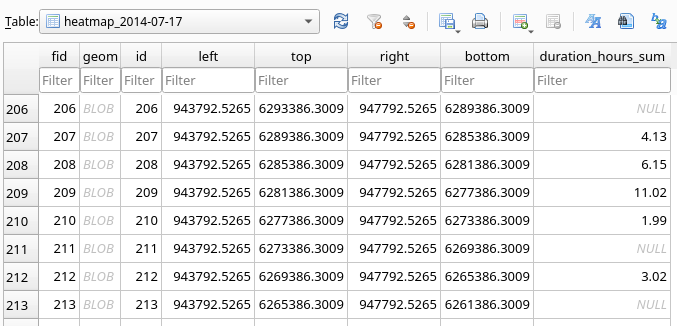
\includegraphics[width=0.8\textwidth,height=8cm,keepaspectratio=true]{content/images/GpkgExample.png}
    \caption{Einträge einer GPKG-Datei}
    \label{fig:GpkgExample}
\end{figure}

Man kann erkennen, dass jede Zeile der Tabelle eine Rasterzelle enthält.
Die Spalten \emph{left}, \emph{top}, \emph{right} und \emph{bottom} enthalten die Begrenzung der Rasterzelle.
Durch den Algorithmus "`Join attributes by location (summary)"' wurde nun noch die letzte Spalte \emph{duration\_hours\_sum} hinzugefügt.
Wie man erkennen kann, enthält diese Spalte \emph{NULL}, wenn sich keine Radarkontrolle in der Rasterzelle befindet.

Als Nächstes müssen die als \acrshort{gpkg}-Datei abgespeicherten Vektordaten in Rasterdaten umgewandelt werden, damit sie später als zweidimensionale numpy-Arrays eingelesen werden können.
Der Unterschied zwischen Vektor- und Rasterdaten kann am besten an GeoTIFF, einem Dateiformat für Rasterdaten, veranschaulicht werden.
Während eine \acrshort{gpkg}-Datei Vektordaten wie Punkte oder Linien speichert, speichert eine GeoTIFF-Datei Pixelwerte wie eine Bilddatei.
Eine weitere Ähnlichkeit zu Bilddateien ist, dass GeoTIFF-Dateien pro Pixel mehrere Kanäle gespeichert werden können.
Im Unterschied zu gewöhnlichen Bilddateien enthält eine GeoTIFF-Datei nach \cite[S. 128]{PracticalGIS} zusätzlich zu den Pixelwerten noch Metadaten, die die räumlichen Eigenschaften des Rasters beschreiben.
Dazu zählen z.\,B. Koordinaten als Georeferenz und das verwendete Koordinatenreferenzsystem.
Damit kann das Raster im Koordinatensystem richtig positioniert werden, ohne dass wie bei \acrshort{gpkg}-Dateien die Grenzen jeder einzelnen Rasterzelle gespeichert werden müssen.
Diese Metadaten werden nach \cite{GeoTIFFStandard} so gespeichert, dass eine GeoTIFF-Datei auch dem \acrshort{tiff}-Format entspricht.
Beispielsweise kann eine GeoTIFF-Datei mit der Bildverarbeitungssoftware \acrfullr{gimp} geöffnet werden, auch wenn es dafür keine wirkliche Anwendung gibt.

Zur Umwandlung der \acrshort{gpkg}-Dateien in GeoTIFF-Dateien kann das Programm \emph{gdal\_rasterize} verwendet werden, welches mit der \acrfull{gdal} mitgeliefert wird.
Den Aufruf dieses Programms sieht man in \autoref{lst:ProcessDatesFunction} in den Zeilen 13 bis 17.
Da \emph{gdal\_rasterize} die Höhe und Breite, sowie die Grenzen des Rasters als Parameter benötigt, werden diese in den Zeilen 6 bis 10 aus der \acrshort{gpkg}-Datei ermittelt.
Wichtig ist auch der Parameter mit der Syntax \emph{[-a attribute\_name]}, der bestimmt, welches Attribut des Vektorlayers für die Zahlenwerte des Rasters verwendet werden soll.
Wie in \autoref{fig:GpkgExample} zu sehen ist, ist dies im vorliegenden Fall \emph{duration\_hours\_sum}.
Ist die GeoTIFF-Datei erstellt, kann diese sehr einfach als numpy-Array eingelesen werden, was in \autoref{lst:GdalOpen} Zeile \ref{gdal_numpy_start} bis \ref{gdal_numpy_end} demonstriert wird.
Außerdem können die Metadaten ausgelesen werden, was in Zeile \ref{gdal_metadata_start} bis \ref{gdal_metadata_end} zu sehen ist.

\begin{minipage}{\textwidth}
\begin{code}
\begin{minted}[
    linenos,
    numbersep=10pt,
    gobble=0,
    frame=lines,
    framesep=2mm,
    escapeinside=!!]{pycon}
>>> from osgeo import gdal

!\label{gdal_numpy_start}!>>> filename = "heatmap_2015-07-02.tif"
>>> geotiff = gdal.Open(filename)
>>> raster_data = geotiff.ReadAsArray()
>>> print(type(raster_data))
<class 'numpy.ndarray'>
>>> print(raster_data.shape)
!\label{gdal_numpy_end}!(50, 50)

!\label{gdal_metadata_start}!>>> geotransform = geotiff.GetGeoTransform()
>>> print(geotransform)
(927793.0, 4000.0, 0.0, 6313386.0, 0.0, -4000.0)
>>> print(f"{geotiff.RasterXSize}x{geotiff.RasterYSize}")
!\label{gdal_metadata_end}!50x50
\end{minted}
\captionof{listing}{Extrahierung der Parameter und Daten aus einer GeoTIFF-Datei}
\label{lst:GdalOpen}
\end{code}
\end{minipage}

Damit ist die Implementierung der Rasterisierung des Datensatzes abgeschlossen.
Die mit \acrshort{gdal} geladenen numpy-Arrays können nun als Input für das neuronale Netz verwendet werden.
Die komplette Implementierung ist in \appendixref{sec:QgisRasterisierung} aufgeführt.


\section{Entwurf eines Modells}
\label{sec:ModellEntwurf}

\section{Experimente}
\label{sec:Experimente}

\section{Ergebnis und Ausblick}
\label{sec:ErgebnisAusblick}


%%%
%%% Nachbau
%%%
\addsec{Literatur}
\renewcommand{\section}[2]{}
\bibliography{citation/quellen}
\clearpage

% Anhänge
\appendix
\addappheadtotoc
\appendixpage
\begin{appendices}
%\include{content/<Name des Anhangs>}

\end{appendices}
\end{document}
